\begin{figure}[htbp]
\centering
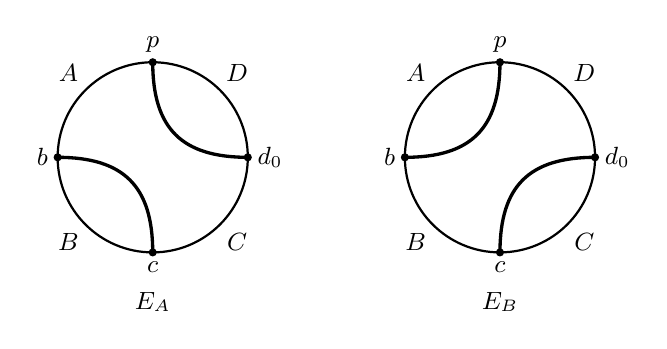
\begin{tikzpicture}[scale=1.05, every node/.style={font=\small}]
\foreach \dx/\ev in {0/{E_{\mathfrak A}},4.2/{E_{\mathfrak B}}}{
  \begin{scope}[xshift=\dx cm]
  \draw[thick] (0,1.15) arc[start angle=90,end angle=450,radius=1.15];
  \foreach \pos/\lab in {(0,1.15)/p,(-1.15,0)/b,(0,-1.15)/c,(1.15,0)/d_0}
    \fill \pos circle[radius=1.4pt];
  \node[above] at (0,1.15) {$p$};
  \node[left] at (-1.15,0) {$b$};
  \node[below] at (0,-1.15) {$c$};
  \node[right] at (1.15,0) {$d_0$};
  \node at (-1.02,1.02) {$A$};
  \node at (-1.02,-1.02) {$B$};
  \node at (1.02,-1.02) {$C$};
  \node at (1.02,1.02) {$D$};
  \node at (0,-1.75) {$\ev$};
  \end{scope}
}
\draw[very thick] (0,1.15) .. controls (0,.35) and (.35,0) .. (1.15,0);
\draw[very thick] (-1.15,0) .. controls (-.35,0) and (0,-.35) .. (0,-1.15);
\begin{scope}[xshift=4.2cm]
\draw[very thick] (0,1.15) .. controls (0,.35) and (-.35,0) .. (-1.15,0);
\draw[very thick] (0,-1.15) .. controls (0,-.35) and (.35,0) .. (1.15,0);
\end{scope}
\end{tikzpicture}
\caption{The two four-port pairings after local caps are attached.
The boundary is drawn as a circle only to show cyclic order; $A,C$
wire $\mathfrak A$ and $B,D$ wire $\mathfrak B$.  Completing around
$A,C$ adds one loop on the left and two on the right.  The thick curves
are open medial strands, not cluster paths.}
\label{four:pairing-figure}
\end{figure}
